% LaTeX Article Template - customizing header and footer
\documentclass{article}

\newtheorem{thm}{Theorem}

% Set left margin - The default is 1 inch, so the following
% command sets a 1.25-inch left margin.
\setlength{\oddsidemargin}{0.25in}

% Set width of the text - What is left will be the right margin.
% In this case, right margin is 8.5in - 1.25in - 6in = 1.25in.
\setlength{\textwidth}{6in}

% Set top margin - The default is 1 inch, so the following
% command sets a 0.75-inch top margin.
\setlength{\topmargin}{-0.25in}

% Set height of the header
\setlength{\headheight}{0.1in}

% Set vertical distance between the header and the text
\setlength{\headsep}{0.2in}

% Set height of the text
\setlength{\textheight}{9in}

% Set vertical distance between the text and the
% bottom of footer
%\setlength{\footskip}{0.15in}

% Set the beginning of a LaTeX document
\usepackage{multirow}
\usepackage{fullpage}
\usepackage{graphicx}
\usepackage{amsthm}
\usepackage{amssymb}
\usepackage{amssymb}
\usepackage{algpseudocode}
\usepackage{caption}
\usepackage{float}
\usepackage{subcaption}
\graphicspath{%
    {converted_graphics/}% inserted by PCTeX
    {/}% inserted by PCTeX
}
%%%%%%%%%%%%%%%%%%%%%%%%%%%%%

\begin{document}\title{Topics on Graphs\\ Spring 2017\\ Math-M330}         % Enter your title between curly braces
\author{Steven Myers}        % Enter your name between curly braces
\date{\today}          % Enter your date or \today between curly braces
\maketitle


% Redefine "plain" pagestyle
\makeatother     % `@' is restored as a "non-letter" character

% Set to use the "plain" pagestyle
\pagestyle{plain}

\section*{Minimum Spanning Trees}
\paragraph{Tree definition}
A \textit{tree} in mathematics or Computer Science is a structure that contains a root node and collection of child nodes. The children nodes are a \textit{recursive} structure that can also contain a collection of children nodes. All nodes except for the root node have exactly one \textit{parent} node. An important property for trees is that trees cannot contain cycles, since every node has exactly one parent. Trees can also be related as a graph. Edges between nodes are the relationship of parent nodes to child nodes in such a representation.

\begin{figure}[H]
    \centering
    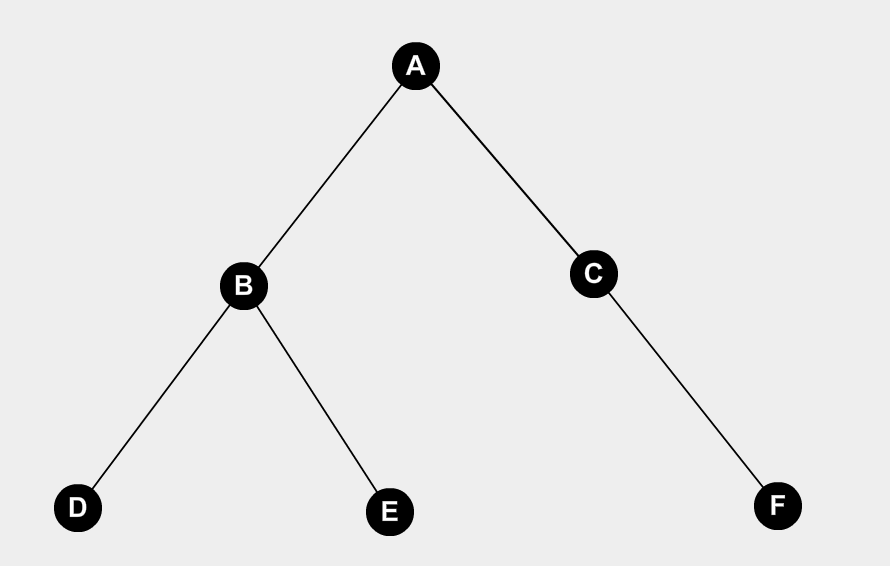
\includegraphics[width=.6\linewidth, height=.25\textheight]{tree_example}
    \caption{A simple tree}
\end{figure}

\paragraph{}
\textit{Spanning trees} are tree structures that are a subsets of an undirected, connected graph. Spanning trees must contain every vertex in a graph while using the minimum number of edges. If the edges of the graph do not have weights (all edges between nodes are equidistant), then we can determine a shortest path between any two nodes in the spanning tree. Consequently, spanning trees are useful in algorithms to determine shortest paths from a starting node to an end node. Spanning trees are useful in real-world applications. For example, it may be desirable for a company to lay cable wires for internet service in such a way that the cable is connected to every residence in an area while using the least amount of wire.

\begin{figure}[H]
    \centering
    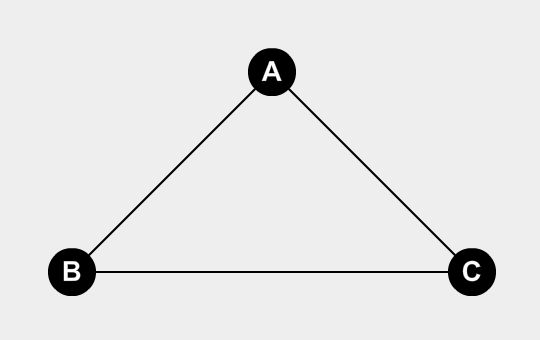
\includegraphics[width=.4\linewidth, height=.2\textheight]{sample_graph}
    \caption{A simple graph}
\end{figure}

\paragraph{}
A graph can have more than one spanning tree. Consider the trivial graph from Figure 2. All of the vertices are share two edges, and no matter how we construct the spanning tree we are able to visit every vertex using exactly two edges. Some spanning tree $T$ is equivalent to a spanning tree $T'$ if both spanning trees visit all of the vertices of the graph in the same minimal number of edges.

\begin{figure}[H]
    \centering
    \begin{subfigure}{.32\textwidth}
        \centering
        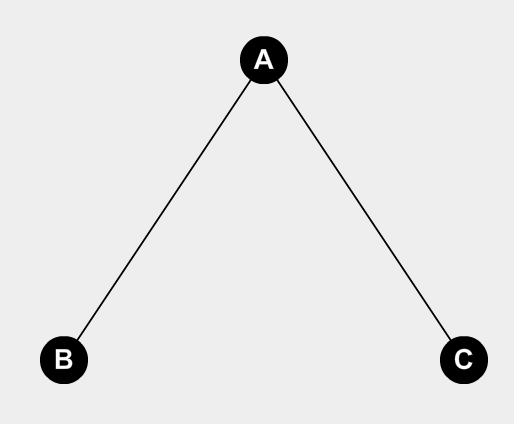
\includegraphics[width=.75\linewidth, height=.2\textheight]{MST1}
    \end{subfigure}
    \begin{subfigure}{.32\textwidth}
        \centering
        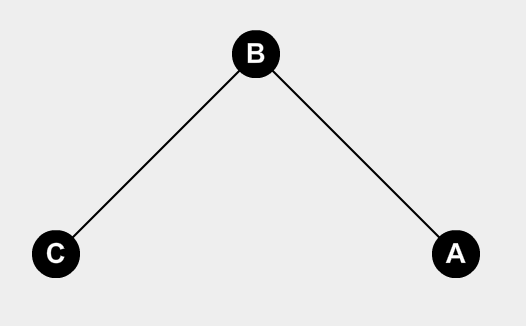
\includegraphics[width=.75\linewidth, height=.2\textheight]{MST2}
    \end{subfigure}
    \begin{subfigure}{.32\textwidth}
        \centering
        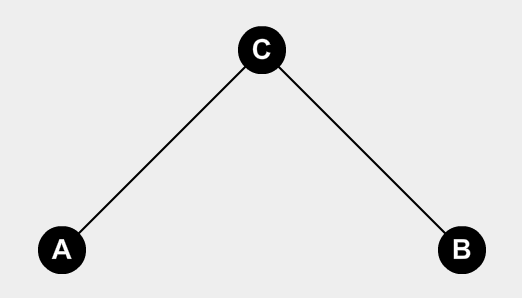
\includegraphics[width=.75\linewidth, height=.2\textheight]{MST3}
    \end{subfigure}
    \caption{Equivalent spanning trees for the graph in Figure 2.}
\end{figure}

\paragraph{}


\medskip

\begin{thebibliography}{9}
\bibitem{wikipedia1}
Wikipedia contributors. "Sierpinski triangle." Wikipedia, \textit{The Free Encyclopedia}. Wikipedia, The Free Encyclopedia, 14 Feb. 2017. Web. 24 Feb. 2017.

\bibitem{wikipedia2}
Wikipedia contributors. "Hausdorff dimension." Wikipedia, \textit{The Free Encyclopedia.} Wikipedia, The Free Encyclopedia, 10 Jan. 2017. Web. 24 Feb. 2017.

\bibitem{online_site}
"Fractal Dimension." \textit{Fractal Foundation Online Course - Chapter 1 - FRACTALS IN NATURE.} N.p., n.d. Web. 24 Feb. 2017.
\end{thebibliography}
\end{document}
